

\documentclass{beamer}

\usepackage{amssymb,amsmath}
\usepackage{graphicx}
\usepackage{url}
\usepackage{color}
\usepackage{pagenote}[continuous,page]
\usepackage{relsize}		% For \smaller
\usepackage{url}			% For \url
\usepackage{epstopdf}	% Included EPS files automatically converted to PDF to include with pdflatex

%For MindMaps
% \usepackage{tikz}%
% \usetikzlibrary{mindmap,trees,arrows}%

%%% Color Definitions %%%%%%%%%%%%%%%%%%%%%%%%%%%%%%%%%%%%%%%%%%%%%%%%%%%%%%%%%
%\definecolor{bordercol}{RGB}{40,40,40}
%\definecolor{headercol1}{RGB}{186,215,230}
%\definecolor{headercol2}{RGB}{80,80,80}
%\definecolor{headerfontcol}{RGB}{0,0,0}
%\definecolor{boxcolor}{RGB}{186,215,230}

%%% Save space in lists. Use this after the opening of the list %%%%%%%%%%%%%%%%
%\newcommand{\compresslist}{
%	\setlength{\itemsep}{1pt}
%	\setlength{\parskip}{0pt}
%	\setlength{\parsep}{0pt}
%}

%\setbeameroption{show notes on top}

% You should run 'pdflatex' TWICE, because of TOC issues.

% Rename this file.  A common temptation for first-time slide makers
% is to name it something like ``my_talk.tex'' or
% ``john_doe_talk.tex'' or even ``discrete_math_seminar_talk.tex''.
% You really won't like any of these titles the second time you give a
% talk.  Try naming your tex file something more descriptive, like
% ``riemann_hypothesis_short_proof_talk.tex''.  Even better (in case
% you recycle 99% of a talk, but still want to change a little, and
% retain copies of each), how about
% ``riemann_hypothesis_short_proof_MIT-Colloquium.2000-01-01.tex''?

\mode<presentation>
{
  \usetheme{CambridgeUS}
  \usecolortheme{dolphin}
  \useoutertheme{default}
  \useinnertheme{default}
  \setbeamercovered{invisible} % or whatever (possibly just delete it)
}
\beamertemplatenavigationsymbolsempty

\usepackage[english]{babel}
%\usepackage[latin1]{inputenc}
\usepackage{subfigure}

\usepackage{times}
\usepackage[T1]{fontenc}
\usepackage{CJKutf8}

%% makes the ppagenote command for figure references at the end.
\makepagenote
\renewcommand{\notenumintext}[1]{}
\newcommand{\ppagenote}[1]{\pagenote[Page \insertframenumber]{#1}}

\title[Experiment Design (01CH740)]{Experiment Design for Computer Sciences (01CH740)}
\author[Claus Aranha]{Claus Aranha\\{\footnotesize caranha@cs.tsukuba.ac.jp}}
\institute[U. Tsukuba]{University of Tsukuba, Department of Computer Sciences}


\title[]{Experiment Design}
\subtitle[]{Lecture 2: Experimentation}
\author[Claus Aranha]{Claus Aranha\\{\footnotesize caranha@cs.tsukuba.ac.jp}}
\institute{Department of Computer Science}

\begin{document}

% Class 2: Experimentation

%% Notes, ``homework''
% Question: What is your research? How do you validate your research?
% Quick review of previous classes: what is science, experiment is one part of science

%% What is an experiment
% Only one part of science, but a very important one
% It is a procedure to observe the world and collect information

%% Possible goals and uses of an experiment 
% Observe the nature as is
% Make one modification and observe the changes
% Carefully control nature, and see how it adapts to your changes

%% This is why it is important to define the goal of the experiment

%% Statistics is an important language to describe an experiment

%% Statistic types of experiments
% Show that a variable is above a certain value
% Show that a variable reaches at least a certain value
% Show that two variables are equivalent

%% Experimental methodology
% Decide the type of experiment
% Decide the factors and their values (which are fixed, which change)
% 

%% Statistical tools for the experiments
% One sided tests, two sided tests
% Normality tests, distribution tests

%% End notes: Repeat homework
% What is your research?
% How do you validate your research?
% What experiments are important for your research?




\section{Pre-class}
\subsection{Opening}

% TODO: Add a cute face in the intro slide
\begin{frame}
  \maketitle
  \begin{center}
    \structure{How was your week?}
  \end{center}
\end{frame}

\begin{frame}
  \frametitle{Last class summary}
  Sorry for being rambly :-)

  \bigskip

  What do you remember from last class?
  
\end{frame}

\begin{frame}
  \frametitle{Last class summary (1)}

  I wanted to focus on four important points:
  
  \bigskip

  \begin{block}{What is science?}    
    \begin{itemize}
    \item Science requires curiosity
    \item Science as a rigorous system 
    \item Science as a community
    \item Science benefitting society 
    \end{itemize}    
  \end{block}
\end{frame}

\begin{frame}
  \frametitle{Last class summary (2)}
  Other important points:
  \bigskip
  \begin{exampleblock}{What is a scientist?}
    \begin{itemize}
    \item Curious about how the world works, How things works
    \item Shares his knowledge with other people
    \end{itemize}
  \end{exampleblock}
  
  \medskip
  
  \begin{alertblock}{Misconceptions about science}
    \begin{itemize}
    \item ``Experiments without guidance''
    \item Just research and nothing else
    \item Common mistakes researchers do (replications, biases, etc)
    \end{itemize}
  \end{alertblock}
\end{frame}

\subsection{Science Communication}
%% TODO: Move this entire part about scientific communication to class one
\begin{frame}
  \frametitle{A day in mercury:}
  \begin{center}
    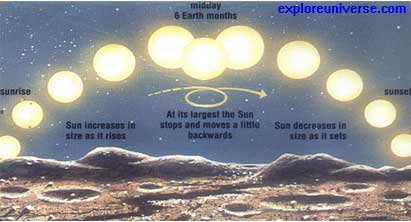
\includegraphics[width=0.8\textwidth]{img/mercuryday}
  \end{center}

  \vfill 

  {\tiny
  Source: http://www.exploreuniverse.com/ic/mercury.html }
\end{frame}

\begin{frame}
  \frametitle{Scientific Communication (1)}

  Two questions for you:

  \begin{enumerate}
  \item<1-> What is the most interesting science related news you have heard recently?
  \item<2-> Where do you get your scientific news?
  \end{enumerate}

\end{frame}

\begin{frame}
  \frametitle{Scientific Communication (2)}

  Start learning something!

  \begin{block}{Podcasts}
    \begin{itemize}
    \item The infinite Monkey Cage -- \url{http://www.bbc.co.uk/podcasts/series/timc} 
    \item Radio Lab -- \url{http://www.radiolab.org/series/podcasts/}
    \item Startalk Radio -- \url{http://www.startalkradio.net/show/the-ig-nobel-prize/}
    \end{itemize}
  \end{block}
\end{frame}

\subsection{Introduction Homework}

\begin{frame}
  \frametitle{Last Week's homework}

  \only<2->{Only one person sent me the research summary... :-(}

  \hspace{1cm}

  \only<3>{Let's try again!}
  
\end{frame}

\begin{frame}
  \frametitle{Homework (for real!)}
    {\small
      \begin{enumerate}
      \item Write an outline of your FIELD (1 or 2 sentences). Write
        it in a way that a non-technical person can understand.

      \item Write an outline of your RESEARCH (1 or 2 sentences)
        inside your field. Write it in a way that a non-technical
        person can understand.


      \item What is the hard part of your research? This question can
        be answered in a technical way.

      \item Think about and describe an experiment that is related to
        your research.
        {\smaller
        \begin{itemize}
        \item Describe the conditions of the experiment (data,
          factors, parameters, etc)
        \item Describe how you evaluate the experiment (when is it
          successful? when does it fail?)
        \item Describe what are possible conclusions for possible experiment results 
        \end{itemize}}
      \end{enumerate}
    }
\end{frame}



\section{Experiment Design}
\subsection{Outline}
\begin{frame}
  \begin{center}
    {\bf Class 2: Experimentalism}
  \end{center}
\end{frame}

\begin{frame}
  \frametitle{Class Outline}
  \begin{itemize}
    \item Last week we talked about how experiments are just a part of science;
    \item But they are a part that many people get wrong;      
  \end{itemize}

  \begin{block}{Idea of this class}
    \begin{itemize}
    \item What is an experiment?
    \item What is an experiment's role in science?
    \item What are the steps needed in experiment design?
    \end{itemize}
  \end{block}    
\end{frame}

\subsection{Definition of Experiment}

\begin{frame}
  \frametitle{What is an experiment?}
  \begin{block}{}
    \begin{center}
      {\small
    An experiment can be characterized as a test (or a series of
    tests), in which changes are introduced in the state of a system
    or process, enabling the observation and characterization of
    effects that can occur as a result of these changes.}
    \end{center}
  \end{block}

  \bigskip

  Common goals of an experiment:
  \begin{itemize}
    \item \structure<2>{Finding out influential variables in a system/process;}
    \item \structure<3>{Determining the desired values for a certain parameter;}
    \item \structure<4>{Characterize the behavior of a system or process;}
  \end{itemize}
\end{frame}

\begin{frame}
  \frametitle{Experiment Characterization} 

  We can define different types of ``experiments'' based on how we
  obtain data from it:

  \begin{exampleblock}{}
    \begin{itemize}
    \item \alert<1>{Retrospective Study;}
    \item \alert<2>{Observational Study;}
    \item \alert<3>{Designed experiment;}
    \end{itemize}
  \end{exampleblock}

  \begin{onlyenv}<1>
  \begin{block}{Characteristics}
    \begin{itemize}
    \item Use of historical data;
    \item Investigating correlations;
    \end{itemize}
  \end{block}
  \begin{block}{Problems}
    \begin{itemize}
    \item Data representativeness;
    \item Availability of data;
    \end{itemize}
  \end{block}
  \end{onlyenv}

\begin{onlyenv}<2>
  \begin{block}{Characteristics}
    \begin{itemize}
    \item Observation of the system with minimal disturbance;
    \item Investigation of usual behaviors;
    \end{itemize}
  \end{block}
  \begin{block}{Problems}
    \begin{itemize}
    \item Low representativeness of extreme cases;
    \item Low variability can affect observation of interesting effects;
    \end{itemize}
  \end{block}
  \end{onlyenv}

\begin{onlyenv}<3>
  \begin{block}{Characteristics}
    \begin{itemize}
    \item Introduction of deliberate changes in the system;
    \item Inference on the \structure{causality} of effects;
    \end{itemize}
  \end{block}
  \begin{block}{Problems}
    \begin{itemize}
    \item Requires rigorous experimental design and data analysis;
    \item Prone to confirmation bias;
    \item Usually more expensive (in cost and time);
    \end{itemize}
  \end{block}
  \end{onlyenv}

\end{frame}




% Outline of an experiment design
% Review: Why do we want to do this?

% First, Take a look at the data. 
% Talk about the many ways to look at the data (Graphs, means, values like that)
% History about the ``person'' dataset
% Maybe the data has been logn'ed? Or passed through some other processing?

% Second, define what kind of experiment you need to do
% List all kinds of experiment variables and decisions (expand from last years class 1 part 2)
% This is probably the longest part

% Third, execute the experiment
% Cares that must be taken when executing the experiment

% Fourth, perform the statistical analysis

%% Omake, some statistic basic notions


\section{Experiment Practices}
\subsection{Characteristics of a good experiment}

\begin{frame}
  \frametitle{Important Principles for experimental research on algorithms}
  \begin{block}{}
    \begin{columns}[t]

      \column{0.4\textwidth}
      \begin{itemize}
        \smaller{
      \item Relevant Experiments;
        \smallskip

      \item Relation to the literature;
        \smallskip

      \item Significant test problems;
        \smallskip

      \item Experimental Design;
        \smallskip

      \item Efficient Implementation;
        }
      \end{itemize}
      \column{0.4\textwidth}
      \begin{itemize}
        \smaller{
        \item Reproducibility;
          \smallskip

        \item Comparability;
          \smallskip

        \item Complete Description;
          \smallskip

        \item Claims supported by results;
          \smallskip
          
        \item Data properly presented.
        }
      \end{itemize}

    \end{columns}
  \end{block}
\end{frame}

%%% 

\subsection{Pre Experimental Design}

\begin{frame}
  \frametitle{Pre Experimental Design (1)}
  
  \begin{block}{}
    Before we begin
  \end{block}
  \begin{itemize}
  \item Do you have all knowledge needed?
    \begin{itemize}
    \item Very common in information sciences
    \item Specific factors/problems in the specific application
    \item Teamwork
    \end{itemize}
    \medskip

  \item<2-> Relevance of the experiment
    \begin{itemize}
    \item Think about the target audience;
    \item Check the literature throughly/avoid reinventing the wheel;
    \item Is the proposed question relevant?
    \item Break down the problem if necessary;
    \end{itemize}
  \end{itemize}
\end{frame}

\begin{frame}
  \frametitle{Pre Experimental Design (2)}

  Decide what is the question you want to answer:

  \begin{block}{Objetives of an experiment}
    \begin{itemize}
    \item Determine the most influential variables in a system;
    \item Determine desired parameter values to reach an output;
    \item Describe the behavior of a system;
    \item Etc.
    \end{itemize}
  \end{block}
  \begin{onlyenv}<2>
    \begin{block}{(some) Types of Experiments}
      \begin{itemize}
      \item Time-series analysis;
      \item Observation of the system;
      \item Planned interference;
      \end{itemize}
    \end{block}
  \end{onlyenv}
\end{frame}

\subsection{Experimental Design}

\begin{frame}
  \frametitle{Experimental Design (1)}
  \begin{block}{Parameter/Factor Selection}
    \begin{itemize}
      {\small
      \item \alert<1>{Educated Guesses}
      \item \alert<2>{One Parameter at a time}
      \item \alert<3>{Factorial Planning}
      }
    \end{itemize}
  \end{block}
  \medskip
  
  {\small
  \begin{onlyenv}<1>
    \begin{itemize}
    \item Arbitrary combination of parameter/values for study;
    \item Observe the behavior; Change some parameters; Repeat;
    \item Risks premature convergence (``good enough'');
    \end{itemize}
    \bigskip
    
    Requires solid knowledge about the underlying problem.
  \end{onlyenv}
  
  \begin{onlyenv}<2>
    \begin{itemize}
    \item Selects and changes one parameter at a time;
    \item Often used, safe;
    \item Unable to determine parameter integration;
    \end{itemize}
    \begin{center}
      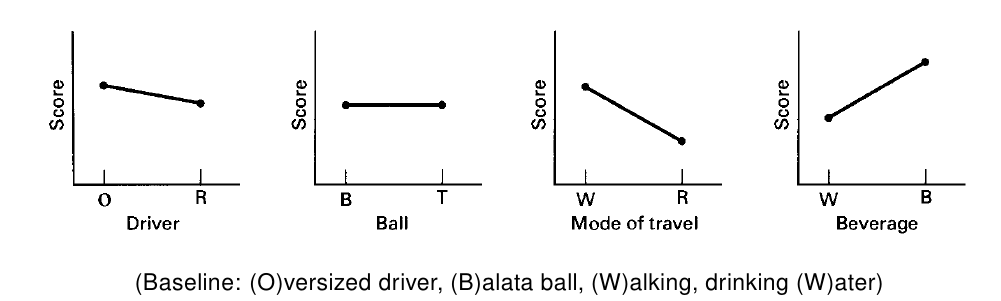
\includegraphics[width=0.7\textwidth]{img/singleparameter}
    \end{center}
  \end{onlyenv}

  \begin{onlyenv}<3>
    \begin{itemize}
    \item Testing the influence of different factors on the system;
    \item Values of each factor are varied in an organized fashion;
    \item Determines individual effects and iteractions;
    \item Experiment size increases with number of factors;
    \end{itemize}
    \begin{center}
      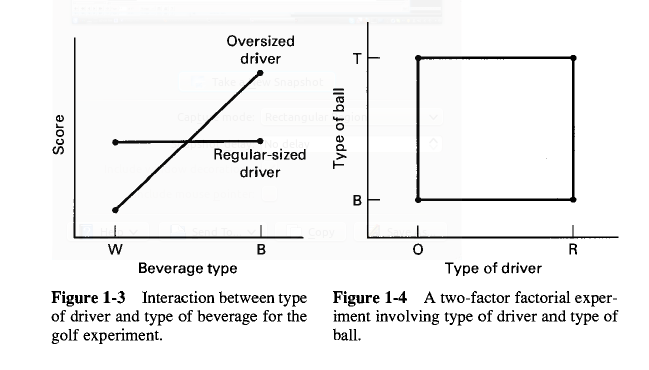
\includegraphics[width=0.5\textwidth]{img/factorialplanning}
    \end{center}
  \end{onlyenv}
  }
\end{frame}

\begin{frame}
  \frametitle{Experimental Design (2)}
  \begin{block}{Data Selection}
    \begin{itemize}
      \item Benchmarks
      \item Natural Data
      \item Random Data
    \end{itemize}
  \end{block}
\end{frame}

\begin{frame}
  \frametitle{Experimental Design (3)}
  \begin{block}{Design Principles}
    \begin{itemize}
      \item \alert<1>{Repetition}
      \item \alert<2>{Randomization}
      \item \alert<3>{Blocking}
    \end{itemize}
  \end{block}

  \begin{onlyenv}<1>
    \structure{Repetition:}\\
    \medskip
    
    \begin{itemize}
      \item {\small Repetition of the experiment allows for estimation of the error}
      \item {\small Used for calculating statistical significance}
      \item {\small Allows for a more precise measure}
      \item {\small Decide beforehand the number of repetitions!}
    \end{itemize}
  \end{onlyenv}

  \begin{onlyenv}<2>
    \structure{Randomization:}\\
    \medskip
    
    \begin{itemize}
    \item {\small Random order of the experiments, Random allocation of
      resources;}
    \item {\small Reduce the bias from data, reduces influence from unrelated
      factors;}
    \item {\small Where randomization is not possible: partial
      randomization, blocking, etc;}
    \end{itemize}
  \end{onlyenv}

  \begin{onlyenv}<3>
    \structure{Blocking:}\\
    \medskip
    
    \begin{itemize}
    \item {\small Removes the influence of unrelated factors}
    \item {\small Breakdown experiments into blocks based on these factors}
    \item {\small Reduces the number of available observations}
    \end{itemize}
  \end{onlyenv}
\end{frame}


\begin{frame}
  \frametitle{Experimental Design (4)}
  \begin{block}{Comparisons}
    \begin{itemize}
      \item Selecting Comparison methods
        \begin{itemize}
        \item Recent Methods;
        \item ``Traditional'' methods;
        \item \alert<2>{Methods Outside your discipline}
        \end{itemize}
      \item Tweaking of Code and Parameter
    \end{itemize}
  \end{block}
\end{frame}


\subsection{Post Experiment}
\begin{frame}
  \frametitle{Statistical Analysis (1)}
  \begin{block}{}
    \begin{itemize}
    \item A good experimental design should give you enough
      information to select the correct statistical
      model.\\ {\tiny (Or close enough)}
      \medskip

    \item Export all possible data from your experiment, use known
      statistical tools to deal with the data\\ {\tiny (Programmers
        have a tendency to reinvent the wheel)}
      \medskip

    \item R, Matlab, Octave, etc...
    \end{itemize}    
  \end{block}
\end{frame}

\begin{frame}
  \frametitle{Statistical Analysis (2)}
  \begin{block}{General Procedure for Hypothesis Testing}
    \begin{enumerate}
      \item<1-> Define the \structure{Null Model} and the desired
        significance level;
      \item<2-> Determine $P(\text{data}|\text{null model})$
      \item<3-> Decide Whether or not to reject the Null Hypothesis
        
        \bigskip

        \only<4> {\small Many people stop here ...}

      \item <5-> Validate the premises of the Statistical Model
      \item <6-> Estimate the \structure{magnititude} of the differences
    \end{enumerate}
  \end{block}
\end{frame}

\begin{frame}
  \frametitle{Analyzing the results}
  \begin{block}{Stick to the Facts!}
    Beware of overgeneralizing the results and making claims not
    supported by the data.
  \end{block}

  \begin{block}{Stick to ALL the facts}
    Avoid cherrypicking the results to make the system look better
    than it is. Complete descriptions are actually more useful.
  \end{block}

  \begin{block}{Dealing with anomalies}
    Any anomalies must be reported, but beware of ``anomaly hunting''.
  \end{block}
\end{frame}

\begin{frame}
  \frametitle{Writing that paper (1)}
  \begin{block}{Be Through}
    Report everything that can help the reader understand the extents
    and limitations of your experiments:
    \begin{itemize}
      \item Stop criterions;
      \item Computational costs (if time, how it was measured);
      \item Parameters, parameter selection methods;
      \item Experimental setup (and its reasoning);
      \item Etc;
    \end{itemize}
  \end{block}
\end{frame}

\begin{frame}
  \frametitle{Writing that paper (2)}
  \begin{block}{Strive for replicability!}
    \begin{itemize}
    \item Be very explicit describing your data
      \begin{itemize}
        \item Cite literature benchmarks;
        \item Algorithms/parameters for artificial data sets;
        \item If hard to obtain, consider distributing your data
          online;
      \end{itemize}
      \medskip

    \item If at all possible, distribute the source code for your
      experiment!\\
      {\tiny make sure you add all information needed for compilation...}
      \medskip

    \item Distribute online experimental data that did not fit the
      paper;
      \medskip

    \item Consider open access models of publication;\\
      {\tiny remember you are usually allowed to distribute pre-prints}
    \end{itemize}
  \end{block}
\end{frame}


\end{document}
